%!TEX root = ../talk.tex

\chapter{Comparison of IoT Business Model}
\markboth{Comparison of IoT Business Model}{}
\chaptauthors{Matthias Diez, Christian Ott, Silas Weber}

\Kurzfassung{
	\begin{itemize}
		\item Explain why IoT and business models for it are relevant
		\item Present the method that is used to gain the results
		\item Summarize the results of the paper
	\end{itemize}
}

\newpage

\minitoc %Das Inhaltsverzeichnis

\newpage
\renewcommand{\labelitemii}{$\diamond$}
\renewcommand{\labelitemiii}{$\circ$}
\section{Introduction and Problem Statement}
	\begin{itemize}
		\item Introduction into the topic
		\item Research Questions / Problem Statement
		\item Structure of Paper
	\end{itemize}

\section{Internet of Things}
	\begin{itemize}
		\item Definition(s) \cite{ju}
		\item Examples of IoT companies
		\item What we understand as IoT in this paper
	\end{itemize}

\section{Business Model Frameworks}
	\begin{itemize}
		\item Definitions \cite{bmc} \cite{dijkman}
			\begin{itemize}
				\item Business 
				\item Business Model 
				\item Business Model Framework
			\end{itemize}
		\item ``Revolutionizing the Business Model'' \cite{gassmann}
			\begin{itemize}
				\item Why design Business Models?
				
				A successful business needs to offer products or sevices that there is a demand for and thus can be sold to make a profit. In short, a business has to create value. A company needs to have a strategy, a way of conducting business on an operational level that will result in long term financial success, else a business is not viable and will disappear from the market sooner or later.
				A business model can be seen as a logical abstraction describing how the business operates to make a profit. A business models hence is a core factor in deciding wheter your business will be driven out of market or prosper. Having a suitable business model is essential. In fact, innovators of business have been found to be 6\% more profitable than product or process innovators (BCG 2008). With the spread of IOT new business models need to be developed to adapt to those technological changes in the environment and seize the opportunities that arise witch such a change. 

				But there seems to be a problem. Few managers can explain their company's business model ad-hoc, let alone define what a business model actually is (Gassman et al.)[1]. They employ a simple conceptualication consisting of four central dimensions: Who, What, How, Value. 

				\item Magic Triangle 
				\begin{itemize}
					\item What is the Magic Triangle?

					The Who, What, How and Value make up the Gassman's magic Triangle. 
					The Who addresses the target customer Group. 
					The What refers to the product or service to those customers. What is the value offered to the customer? 
					The How addresses the process and acitivties as well as the resources and capabilities that are required for building and distributing the value propositions.
					The Value explains how the business model is financially viable. How is the value generated? It includes cost and revenue structures.
					
					
						\begin{figure}[ht]
						    \begin{center}
						    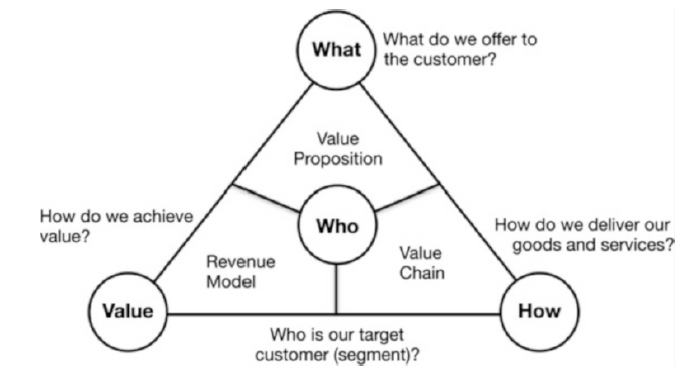
\includegraphics[scale=0.6]{Talk11/Figure1.png}
						    \end{center}
						    \caption{the magic triangle}
						    \label{label}
						\end{figure}

					Figure 1.1 shows the constellation of the magic triangle with the ``Who'' node in the middle.
					Gassman aruges that reducing the busniness model to those four components allows for a simple, yet thorough enogh view of the business model architecture.



				\end{itemize}
				\item Creating new Business Model

				Creating new business models is not an easy task. It requires thinking outside the box, going beyond convention industry philosophy and can quickly become complex. People that are versed in change managment will recognize some of the problem. First, why even come up with a new or improved business model? As long as there are still profits coming in, why take a risk and leave your comfort zone? Competion and environmental factor are always in movement. What works today may not work so well anymore in a few years. The syndrome known as the boiling frog syndrome states that gradually increasing problems are go unnoticed and or not dealt with until until it's too late to tackle them. A frog in pot with water won't jump out if the water is slowly brought to boil and when the water gets too hot for him, his muscles are too weak to jump out. Likewise, a business that has diminishing returns year after year may not be concerned about the the little loss between consective year. But when they realize the devasting loss sufferd over multiple years there aren't any resources left to tackle the problem and they go bankrupt.

				Another problem is the not invented here syndrome, meaning that ideas not coming from within the company are disregarded soley beacause they come from the outside. As a consequence, business models should not just be copied from somewhere else but rather bring in external stimuli when generating ideas from within.

				Gassman analyzed 250 business models in differnt industries from the last 25 years and as a result identified 55 pattern of business models that have served as the basis for new business modles in the past. Then, togheter with selected companies they developed a construction methodology based on the fact that 90\% of all new business models have recombined previousley existing ideas, concpets and  technologies.

				The BMI Navigator is the ready-to-use methodology for coming up with new business models consisting of the following three steps:

				\begin{itemize}
					\item Initiation

					Describing the current business model is a good starting point. It creates a common ground for discussing the things that are done well and what needs improvement, and opportunities are open to be exploited. Also it get the participants started thinking in the ways of business models.
					Open-minded team members are essential, preferably from different functions. This allows different viewpoint and thinking outside the box as well as overcoming the prevailing industry logic.

					\item Ideation

					Recombining existing ideas helps generating new busniness models. Gassman  condensed for this puropose the 55 business models into a set of pattern cards as shown in figure 1.2. Each card has a title, a description and an example. The goal is applying differnt cards to the current model to see what would change in this situation. The cards should trigger discussions and act as a stimuli for new innovative ideas.

					\begin{figure}[ht]
						    \begin{center}
						    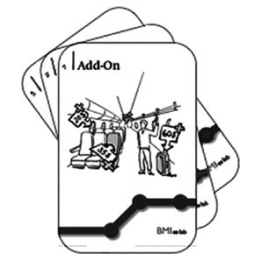
\includegraphics[scale=0.6]{Talk11/Figure2.png}
						    \end{center}
						    \caption{pattern card}
						    \label{label}
						\end{figure}



					\item Integration

					The last step is the integration. It's obvious that a newly genearated idea cannot be implemented instantaneously. New ideas need to be gradually fleshed out into fully operational business models. Considering the new stakeholders, partners and consequences for the market is crucial.


				\end{itemize}
			\end{itemize}
		\item ``Business Model Canvas'' \cite{bmc}
			\begin{itemize}
				\item What is the canvas used for? How was it developed? How relevant is this framework?
				\item Explain nine Building Blocks
				\begin{itemize}
					\item Value Proposition
					\item Customer Segments
					\item Channels
					\item Customer Relationships
					\item Key Activities
					\item Key Resources
					\item Key Partners
					\item Revenue Streams
					\item Cost Structures
				\end{itemize}
			\end{itemize}
	\end{itemize}
\section{Available IoT Business Model Frameworks}
	\begin{itemize}
		\item Explain changes in Business Models due to IoT Development
			\begin{itemize}
				\item From ``Business models for the Internet of Things'' \cite{dijkman}
				\begin{itemize}
					\item Explains typical types for the Business Model Canvas building blocks for IoT companies
				\end{itemize}
				\item From ``Designing Business Models for the Internet of Things'' \cite{westerlund}
				\begin{itemize}
					\item Explains how ecosystem business models can be designed (Value Design) to show ``the dynamics between the components'' or ``ow the engine works''

					\begin{enumerate}[I]
						\item \textbf{Value Drivers}
						\begin{itemize}
							\item Individual motivations
							\item Shared motivations
						\end{itemize}
						\item \textbf{Value Nodes}
						\begin{itemize}
							\item Actors
							\item Activities
							\item (Automated) processes
						\end{itemize}
						\item \textbf{Value Exchanges}
						\begin{itemize}
							\item Resources
							\item Knowledge
							\item Money
							\item Information
						\end{itemize}
						\item \textbf{Value Extracts}
						\begin{itemize}
							\item Monetization
						\end{itemize}					
					\end{enumerate}
				\end{itemize}
				\item From ``IEEE-SA Internet of Things (IoT) Ecosystem Study'' \cite{cisco}
					\begin{itemize}
						\item IoT Ecosystem
							\begin{enumerate}[I]
								\item \textbf{Where does IoT stand today}
									\begin{itemize}
										\item Players
										\item Market
										\item Technology
										\item Standardization
									\end{itemize}
								\item \textbf{Business Model View}
									\begin{itemize}
										\item New segments
										\item Open issues / Insufficiency
									\end{itemize}		
							\end{enumerate}
					\end{itemize}
				\item From ``Business Models and the Internet of Things'' \cite{fleisch}
					\begin{itemize}
						\item Based on 55 different business models patterns \cite{gassmann}
						\item IoT Business Model 1: Digitally Charged Products
							\begin{itemize}
								\item A digitally charged product ``links digital services to physical products to create a hybrid bundle that is a single whole.''
								\item \textbf{Components}
									\begin{enumerate}[a]
										\item Business Model View
										\item Physical Freemium
										\item Digital Add-on
										\item Digital Lock-in
										\item Object Self Service
										\item Remote Usage and Condition Monitoring
									\end{enumerate}
							\end{itemize}
						\item IoT Business Model 2: Sensor as a Service
							\begin{itemize}
								\item A sensor as a service business model is based on ``collecting, processing and selling for a fee the sensor data [...]''.
							\end{itemize}
					\end{itemize}
			\end{itemize}
	\end{itemize}

\section{Comparison of available IoT Business Model Frameworks}
	\begin{itemize}
		\item Text with explanations of differences between frameworks in Chapter 5
		\item If applicable: Comparison table along different attributes
		\item Introduction into case company (fictitious example)
		\item Present model of case company for each framework
	\end{itemize}

\section{Evaluations and Discussion}
	\begin{itemize} 
		\item Partly based on outcome of discussion within the seminar
		\item Critical questions regarding the relevance of the results
		\item How can the conducted comparison help IoT companies to design better business models?
	\end{itemize}

\section{Summary and Conclusions}
	\begin{itemize} 
		\item Summarize the paper content
		\item Show limitations of the paper
		\item Give indications for potential future work related to the topic of this paper
	\end{itemize}

	 \begin{thebibliography}{99}
 		 \bibitem {gassmann} O. Gassmann, K. Frankenberger, and M. Csik: \emph{Revolutionizing the business model.} in O. Gassmann and F. Schweitzer (Eds.), Management of the Fuzzy Front End of Innovation. Springer, New York, pp. 89-97, 2014, \url{http://link.springer.com/chapter/10.1007%2F978-3-319-01056-4_7}, last visit: October 06, 2016.

 		 \bibitem {bmc} Strategyzer AG: \emph{The Business Model Canvas}, \url{http://www.businessmodelgeneration.com/canvas/bmc}, last visit: October 06, 2016.

 		 \bibitem {dijkman} R.M. Dijkman, B. Sprenkels, T.Peeters, and A. Janssen: \emph{Business Models for the Internet of Things}, International Journal of Information Management, Vol 35, pp 672-678, 2015.

 		 \bibitem {fleisch} E. Fleisch, M. Winberger, F. Wortmann: \emph{Business Models and the Internet of Things}, Bosch Internet of Things \& Services Lab, pp 1-19, August 2014, \url{http://www.iot-lab.ch/?page_id=10543}, last visit: October 06, 2016.

 		 \bibitem {rossi} B. Rossi: \emph{How the Internet of Things is Changing Business Models}, Information Age - Insight and analysis for IOT leaders, May 4, 2016 \url{http://www.information-age.com/it-management/strategy-and-innovation/123461371/how-internet-things-changes-business-models}, last visit: October 06, 2016.

 		 \bibitem {hui} G. Hui: \emph{How the Internet of Things Changes Business Models}, Harvard Business Review, July 24, 2014, \url{https://hbr.org/2014/07/how-the-internet-of-things-changes-business-models}, last visit: October 06, 2016.

 		 \bibitem {cisco} CISCO: \emph{IEEE-SA Internet of Things Ecosystem Study}, IEEE Standards Association, New York, 2015, \url{http://www.cisco.com/c/dam/en/us/solutions/collateral/industry-solutions/dlfe-670918525.pdf}, last visit: October 06, 2016.

 		\bibitem {westerlund} M. Westerlund, S. Leminen and M. Rajahonka: \emph{Designing Business Models for the Internet of Things} Technology Innovation Management Review, July 2014, \url{http://timreview.ca/article/807}, last visit: October 06, 2016.

 		\bibitem {ju} Jaehyeon Ju, Mi-Seon Kim and Jae-Hyeon Ahn: \emph{Prototyping Business Models for IoT Service}, Procedia Computer Science, 91, pp. 882 - 890, 2016, \url{http://www.sciencedirect.com/science/article/pii/S1877050916312911}, last visit: October 06, 2016.
	 \end{thebibliography}


% Je nach Talk Nummer wird ausschließlich im jeweiligen \texttt{TalkX} Verzeichnis
% gearbeitet. Bitte Dateien, Bilder etc. \textbf{nur} im Verzeichnis \texttt{TalkX}
% ablegen und bearbeiten. Die Ausarbeitung wird in die jeweilige
% \texttt{Seminar-Arbeit.tex} geschrieben. Bitte die Datei \texttt{Example.tex} als 
% Grundlage nehmen. Formatierungen, Seiteneinstellungen oder die Datei \texttt{talk.tex} 
% dürfen nicht geändert werden.

% Sollte es sich absolut nicht vermeiden lassen, daß weitere usepackages
% eingebunden werden müssen o.ä. bitte \textbf{niemals} die Datei
% \texttt{talk.tex} bearbeiten. Dafür vorgesehen ist die Datei
% \texttt{TalkX/MyHeader.tex}. Bitte nur im Notfall bzw. nach
% Rücksprache mit dem Betreuer von dieser Möglichkeit Gebrauch machen,
% da \LaTeX \ nicht über Namensräume verfügt und sich somit Konflikte zwischen
% einzelnen Paketen ergeben können.

% \section{Gliederung der Arbeit}

% Die Seminar-Arbeit wird in ein Kapitel (\texttt{$\backslash$chapter}) geschrieben. 
% Zur Gliederung der Arbeit werden die Befehle
% \texttt{$\backslash$section\{\}},
% \texttt{$\backslash$subsection\{\}}, und
% \texttt{$\backslash$subsubsection\{\}}
% verwendet.

% Absätze müssen generell mit einer leeren Zeile getrennt werden und nicht mit
% \texttt{$\backslash$$\backslash$} oder \texttt{$\backslash$newline}. 
% Bitte die Befehle \texttt{$\backslash$newpage}, \texttt{$\backslash$clearpage} etc. nicht verwenden.

% Aufzählungen mit und ohne Nummerierung können mit den folgeneden Befehlen erstellt werden:
% \begin{quote}
%   \begin{verbatim}
%   \begin{enumerate}
%     \item ...
%     \item ...
%   \end{enumerate}

%   \begin{itemize}
%     \item ...
%     \item ...
%   \end{itemize}
%   \end{verbatim}
% \end{quote}

% Für Beschreibungen kann der folgende Befehl benutzt werden:
% \begin{quote}
%   \begin{verbatim}
%   \begin{description}
%     \item[Begriff] Beschreibung
%     \item[Begriff] Beschreibung
%   \end{description}
%   \end{verbatim}
% \end{quote}


% \section{Bilder und Tabellen}

% Bitte \textbf{alle} Bilder ohne Dateinamenendung einbinden und das jeweilige
% Bild als \texttt{.jpg} oder \texttt{.pdf} im Verzeichnis \texttt{TalkX} ablegen. 
% Zum Einbinden kann der folgende Befehl verwendet werdet:
% \begin{quote}
%   \begin{verbatim}
%   \begin{figure}[ht]
%     \begin{center}
%     \includegraphics[scale=0.6]{TalkX/filename}
%     \end{center}
%     \caption{Beschriftung}
%     \label{label}
%   \end{figure}
%   \end{verbatim}
% \end{quote}

% \begin{figure}[ht]
% 	\begin{center}
%   \includegraphics[scale=0.6]{Example/uzh_logo_d}
%   \end{center}
%   \caption{Beschriftung}
%   \label{fig:label}
% \end{figure}

% Beim Einbinden den relativen Pfad angeben und keinen absoluten!
% Anstatt \texttt{[scale=0.6]} können auch die Parameter \texttt{[width=4cm]} oder
% \texttt{[width=0.6$\backslash$textwidth]} für die Skalierung der Bilder verwendet werden.
% In der schriftlichen Ausarbeitung müssen die Bilder mit einer Mindestauflösung
% von 600dpi erstellt werden.

%   \begin{table}[h]
%     \caption{Beschriftung}
%     \label{tab:label}
%   	\begin{center}
%     \begin{tabular}{|c|c|c|c|} \hline
% 	          & A & B & C \\ \hline\hline
% 	        X & 1 & 2 & 3 \\ \hline
% 	        Y & 4 & 5 & 6 \\ \hline
% 	        Z & 7 & 8 & 9 \\ \hline
% 	  \end{tabular}
% 	  \end{center}
%   \end{table}

% Die Tabelle \ref{tab:label} kann z.B. mit dem folgenden Befehl erstellt werden:
% \begin{quote}
%   \begin{verbatim}
%   \begin{table}
%     \caption{Beschriftung}
%     \label{tab:label}
%     \begin{center}
%     \begin{tabular}{|c|c|c|c|} \hline
% 	          & A & B & C \\ \hline\hline
% 	        X & 1 & 2 & 3 \\ \hline
% 	        Y & 4 & 5 & 6 \\ \hline
% 	        Z & 7 & 8 & 9 \\ \hline
%     \end{tabular}
%     \end{center}
%   \end{table}
%   \end{verbatim}
% \end{quote}

% Die Bilder und Tabellen müssen grundsätzlich mit einer Beschriftung (\verb|\caption|)
% versehen werden, und im Text mit \texttt{$\backslash$ref\{label\}} referenziert werden.
% Das \texttt{caption} ist bei Bildern grundsätzlich unten und bei Tabellen oben!


%\section{Literaturverzeichnis}

% Am Ende des Kapitels wird das Literaturverzeichnis erstellt. Bei den Bibitems
% wird \textbf{keine} Marke angegeben, es werden die automatisch erzeugten
% Marken [1],[2],... verwendet. Bei einer Referenz müssen grundsätzlich die
% Autoren, der Titel, der Verlag und das Erscheinungsdatum in dem folgenden Format 
% angegeben werden:
%\begin{verbatim}
%	\bibitem {label} N. Author: Title of the document; Type of document 
%   (technical report, deliverable, Workshop/Conference Name ...), 
%   (Location, Vol. X, No. Y), Month, Year, pages, URL (if available).

%	\bibitem {label} Website title; \url{Website URL}, Month, Year of last visit.
%\end{verbatim}
% Wenn in der Referenz eine Internetadresse benutzt wird, muss diese mit dem
% Befehl \texttt{$\backslash$url\{http://...\}} angegeben werden.

% Im Text werden die Bibitems mit \texttt{$\backslash$cite\{label\}} referenziert.
% Für alle verwendeten Arbeiten und Bilder müssen an der jeweiligen Stelle Referenzen
% eingefügt werden.

% Eine ausführliche Anleitung zur Referenzierung in wissenschaftlichen Arbeiten 
% findet sich im \emph{Leitfaden zur Erstellung schriftliche Seminararbeiten} \cite{leitfaden}. 

% \section{Kompilieren}

% \LaTeX \ ist bei allen gängigen Linux Distributionen dabei. Unter Linux wird 
% das Dokument mit \texttt{pdflatex talk.tex} im Hauptverzeichnis kompiliert, 
% was die Datei \texttt{talk.pdf} erzeugt. 

% Für Windows ist die \TeX \ Implementation, MiKTeX (\url{http://www.miktex.org/}) zusammen mit dem \LaTeX \ Tool, TeXnicCenter (\url{http://www.toolscenter.org/}) zu empfehlen.

% Probleme, Anregungen und Fragen bzgl. der Anfertigung des Dokumentes richten
% Sie bitte per Email an die Betreuer.

% Zum Abgabetermin ist es dann nur notwendig das Verzeichnis
% \texttt{TalkX} zu packen (mit \texttt{zip} oder \texttt{tar}) und per
% Email an die Betreuer zu senden.


